\documentclass[a4paper,10pt]{article}
\usepackage[paper=a4paper, hmargin=1.5cm, bottom=1.5cm, top=3.5cm]{geometry}
\usepackage[T1]{fontenc}
\usepackage{fancyhdr}
\usepackage{lastpage}
\usepackage{xspace}
\usepackage{xargs}
\usepackage{ifthen}
\usepackage{caratula}
\usepackage{changepage}
\usepackage{qtree}
\usepackage{algorithmicx, algorithm}
\usepackage[noend]{algpseudocode}
\usepackage{amsmath}
\usepackage{graphicx}
\usepackage{subcaption}
\graphicspath{ {images/} }

\usepackage[colorlinks=true, linkcolor=blue]{hyperref}
\usepackage[utf8]{inputenc}

\hypersetup{%
 % Para que el PDF se abra a página completa.
 pdfstartview= {FitH \hypercalcbp{\paperheight-\topmargin-1in-\headheight}},
 pdfauthor={Nicolás Ansaldi},
 pdfkeywords={},
 pdftitle={Algoritmos y Estructuras de Datos III – TP1},
 pdfsubject={TP1}
}

%%%%%%%%%%%%%%%%%%%%%%%%%%%%%%%%%%%%%%%%%%%%%%%%%
% PARAMETROS A SER MODIFICADOS
%%%%%%%%%%%%%%%%%%%%%%%%%%%%%%%%%%%%%%%%%%%%%%%%%

%cuatrimestre de acuerdo a la opcion
\newcommand{\Cuatrimestre}{$2^\mathrm{er}$ cuatrimestre de 2017}

%%%%%%%%%%%%%%%%%%%%%%%%%%%%%%%%%%%%%%%%%%%%%%%%%
% OTRAS OPCIONES QUE NO HAY QUE MODIFICAR
%%%%%%%%%%%%%%%%%%%%%%%%%%%%%%%%%%%%%%%%%%%%%%%%%

% Acomodo fancyhdr.
\pagestyle{fancy}
\thispagestyle{fancy}
\lhead{Algoritmos y Estructuras de Datos III}
\rhead{\Cuatrimestre}
\cfoot{\thepage /\pageref{LastPage}}
\renewcommand{\footrulewidth}{0.4pt}
\setlength{\headheight}{13pt}


\begin{document}

% Estos comandos deben ir antes del \maketitle
\materia{Algoritmos y Estructuras de Datos III} % obligatorio
\submateria{Segundo Cuatrimestre de 2017} % opcional
\titulo{Trabajo Práctico 1} % obligatorio
\subtitulo{} % opcional
\grupo{} % opcional 

\integrante{Nicolás Ansaldi}{128/14}{nansaldi611@gmail.com} % obligatorio 

\maketitle

% compilar 2 veces para actualizar las referencias
%\tableofcontents

\pagebreak

\tableofcontents

\newpage

\section{Backtracking}

\subsection{Descripcion del problema}

	El problema consiste en formar el grupo más grande de agentes comfiables para esto se cuenta con una tabla que representa las encuestas hechas a los agentes. La primera columna de dicha tabla representa el agente encuestado mientras que la segunda columna representa lo que dicho agente informó. Además, cada agente puede elegir informar algo como no, y si lo hace puede hacer tantas declaraciones como desee. Luego la tabla puede ser vacía como tener muchas entradas (notar que la tabla no puede ser infinita). Una vez hechas todas las encuestas se procede a decir cuál es el grupo más grande de agentes confiables. No todo conjunto de agentes es válido por lo que hay ciertas propiedades que tiene que cumplir. La primera es que si un agente dentro del conjunto confía en otro agente, ese agente también debe estar en el grupo, la segunda es que si un agente dentro del conjunto desconfia de otro agente, este no puede ester en el conjunto. Algunos ejemplos serían:
	
\begin{table}[H]
\begin{tabular}{c c}
Agentes & Encuestas  \\ [0.5ex]
\hline
1 & 2 \\
2 & 3 \\
3 & -1 \\
0 & 0 \\ [1ex]
\hline
res: 2 \\
\end{tabular}
\end{table}

\begin{table}[h]
\begin{tabular}{c c}
\centering
Agentes & Encuestas \\ [0.5ex]
\hline
1 & 5 \\
2 & 3 \\
3 & 4 \\
5 & -1 \\ [1ex]
\hline
res: 3 \\
\end{tabular}
\end{table}

\subsection{Solución Propuesta}

	La idea para resolver este problema es considerar todos los posibles casos. Para esto vimos que cada agente puede estar como no en el conjunto, o sea, se va a analizar ambos conjuntos resultantes, uno donde el agente esté en el conjunto y otro donde no esté. A la hora de agregar un agente, llamémoslo i, al conjunto primero vemos que se pueda, esto significa que va a seguir siendo un conjunto válido, para esto vamos a ver un par de cosas. La primera es que nadie en el conjunto desconfíe de i, luego veremos que i no desconfíe de nadie que está en el conjunto, también se verifica que la encuesta del agente tenga sentido lógico, o sea, que no desconfíe de si mismo y, como puede hacer más de una declaración, que no desconfie y confie de un agente. Además para la rama en la cuál no se agrega al agente vereficamos que tenga sentido que no este en el conjunto, esto es que nadie, que este en el conjunto, confie en él. Una vez hecho esto, y  para los otros posibles conjuntos válidos, se elegirá el conjunto con mayor cantidad de agentes. 
	
\subsection{Resolución}
	La técnica de backtracking consiste en pensar conceptualmente en un árbol que contega todas las posibles soluciones. Por esto la solución que propone mi algoritmo es la siguiente:
	
\begin{itemize}
\setlength\itemsep{-0.2em}
\item Partir de la raíz (ningún agente elegido).
\item Comenzar por el primer agente ver si puede ser agregado al conjunto (las consideraciones descriptas en el punto anterior) y considerar que no forme parte del mismo, luego recorrer recursivamente cada una de esas 2 posibilidades para el elemento siguiente (2 ramas).
\item A partir del segundo elemento, recorrer recursivamente cada una de las 2 ramas sólo si ésta es válida, en otras palabras, si puede ser agregado el agente al conjunto. Además si el agente tiene que estar en el conjunto (porque alguien en el conjunto confía en él) la rama que corresponde a no agregar al agente no se recorre ya que no sería una instancia válida del problema.
\item Al llegar a una hoja que esté en el último nivel (cuando la altura del árbol es igual a la cantidad de agentes) se chequea que el conjunto resultante sea válido esto lo hacemos por que a la hora de agregar un agente al conjunto no estamos viendo que si este confia en alguien que no esta en el conjunto se pueda agregar a ese agente en el futuro. Luego si la cantidad de agentes dentro del conjunto resultante es mayor a la que ya tenés, entonces ésta será la mejor solución. Si no, entonces me quedo con la solución que tenía antes.
\end{itemize}
	
\subsection{Pseudocódigo}

\begin{algorithm}[H]
\caption{Backtracking}\label{Ej1}

\begin{algorithmic}[H]
\Procedure{Backtracking}{vector(pair(agente, agente)) encuestas, agentes, ConjAgentes}
\If{Si no me quedan agentes para evaluar}
\If{longitud(ConjAgentes) > solucion}
\State solucion $=$ longitud(ConjAgentes)
\EndIf
\EndIf
\If{PuedoAgregarAgente}
\State Paso Recursivo rama agregueAlAgente
\EndIf
\If{NadieConfiaEnElAgente}
\State Paso Recursivo rama NoAgregoAlAgente
\EndIf
\EndProcedure
\end{algorithmic}
\end{algorithm}

	A la hora de recorrer ambas ramas, se verifica que no genere instancias inválidas. Lo que hacen las guardas de los ifs es comprobar esa validez.
\subsection{Demostración de correctitud}

	La técnica descripta anteriormente parte de pensar al problema como un árbol con todas las posibles soluciones. Cada nodo del árbol representa como se va ir modificando nuestro conjunto incluyendo o no a un determinado agente. A pesar de que nuestro algoritmo se basa en esta idea falta decir porque es correcto respecto a nuestro problema ya que como dijimos antes no recorre todos los casos. La razón es que recorre las ramas que son válidas según las condiciones del problema y no considera las inválidas. Una vez que tenemos el conjunto de soluciones posibles se queda con la mejor de ellas, en este paso (cuando ya se recorrió todo el árbol) se podrían considerar las soluciones descartadas pero serían descartas de nuevo, ya que no cumplen con lo pedido, lo que hacemos es descartalas antes de llegar al final del árbol para ahorrarnos recorrer dichas ramas. Entonces al final generamos todas las posibles soluciones y nos quedamos con la mejor.

\subsection{Complejidad teórica}
	
	Como dijimos antes la idea conceptual del problema es pensarlo como un árbol de soluciones. Como este árbol contempla todas las posibles soluciones es un árbol completo, ya que por cada nodo tenemos 2 opciones, que forme parte del conjunto o que no forme (no hace falta considerar cuando alguna rama no es recorridas ya que estamos considerando complejidad en peor caso, por lo que  consideramos el árbol completo). Entonces terminamos teniendo un árbol con $2^{i}$ hojas, donde "i" es la cantidad de agentes. Además para pasar de un nivel del árbol a otro, pagamos O($a^{2}*i$) esto se debe a que vemos las encuestas del agente evaluado y las encuestas de los agentes que ya pertenecen al conjunto y chequeamos que cumplan lo descripto anteriormente. Esto lo hacemos cuando queremos ver si un agente es confiable, para la rama que no es confiable pagamos O($a$) para ver si efectivamente el agente evaluado puede no pertenecer al conjunto, luego nos queda la suma de las complejidades O(($a^{2}*i$) + ($a^{2}*i$)) donde nos quedamos con la más grande. Luego en el último nivel hacemos un chequeo para ver si efectivamente el conjunto es válido, esto se debe a que a la hora de agregar un agente al conjunto no estamos considerando que si éste confía en un agente y ese agente no se encuentra en el conjunto lo pueda agregar en el futuro. Para hacer esto tenemos que recorrer una vez mas el conjunto y ver que siga siendo un conjunto válido. Esto nos toma O($i^{2}a$) pasos. Luego, una vez recorrido todo el árbol, terminamos teniendo una complejidad de O($2^{i}*((i*a^{2})+(i^{2}*a))$) = O($2^{i}*(max(i*a^{2}, i^{2}*a))$).
	
\subsection{Experimentación} 
	
	Para analizar la performancia del algoritmo decidimos considerar diferentes entradas. Cada entrada consiste en fijar la cantidad de agentes (yendo desde 1 agente hasta 23) y tomar 100 repeticiones para la cantidad fijada. Cada repetición toma una cantidad de encuestas random (yendo desde 1 hasta 31). Entonces, por ejemplo, tenemos 100 repeticiones (cada una con una cantidad aleatoria de encuestas) para un agente, luego 100 repeticiones para 2 agentes y asi sucesivamente, una vez tomadas todas las muestras se corre el algoritmo utilizandolas y se toma el tiempo que tarda, y una vez que se tienen los tiempos se toma un promedio de las 100 muestras. Las entradas que consideramos fueron, una donde todas las encuestas son positivas, una donde todas las encuestas son negativas y por último una donde se elige aleatoriamente si la encuesta es positiva o negativa.       
	
\begin{figure}[h]
\begin{subfigure}{0.5\textwidth}
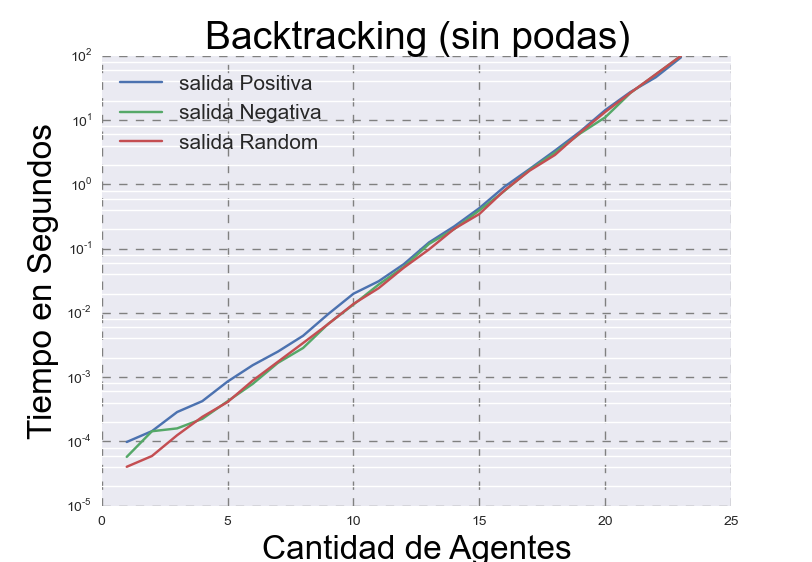
\includegraphics[scale=0.45]{BacktrackingLog.png}
\end{subfigure}
\begin{subfigure}{0.5\textwidth}
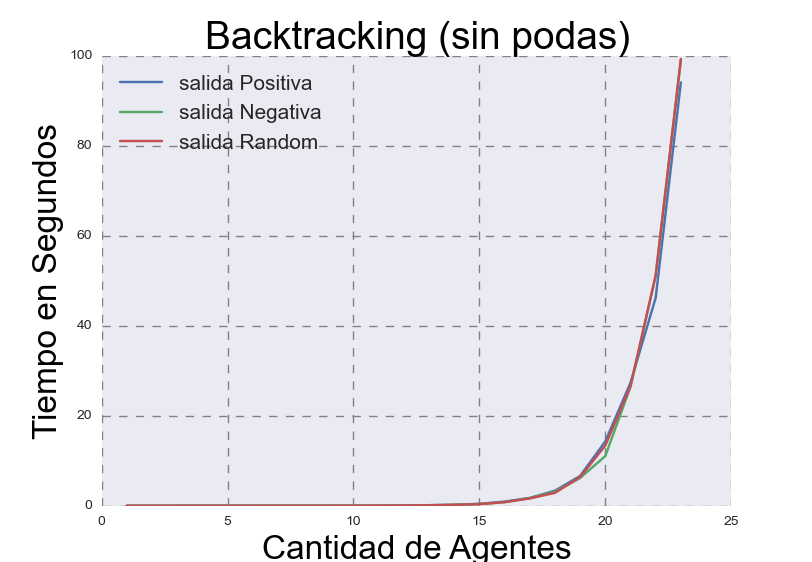
\includegraphics[scale=0.45]{Backtracking.png}
\end{subfigure}
\end{figure}

	En el gráfico podemos ver que el algoritmo se comporta de una manera similar para las 3 entradas, esto se debe que estamos recorriendo la mayoría de soluciones, o sea, estamos recorriendo casi todo el árbol. 
	





\newpage 

\section{Backtracking (Podas)}

	La descripción del problema como la forma de pensarlo son las mismas que el ejercicio anterior.

\subsection{Resolución}
	
	Además de lo dicho en el ejercicio anterior, la idea es podar más el árbol para no recorrer ramas donde no nos interese su solución o sea un caso inválido. Para esto tenemos 2 podas, la primera consiste en no ramas que no mejoren mi mejor solución hasta el momento y la segunda consiste en hacer un análisis a futuro de la confiabilidad de los agentes. Para la primera consideremos un conjunto con "k" elementos en el, "a" representa la cantidad total de agentes e "i" representa los agentes que ya fueron evaluados, la poda consiste en que si $k+(a-i)$ <= s (notar que "a-i" representa los agentes que faltan por evaluar), donde s es la mejor solución hasta el momento, si esto pasa no seguimos recorriendo esa rama ya que no aporta nada mejor a lo que tenemos. La otra consiste en hacer un mejor chequeo de la confiabilidad. Además de lo descripto en el ejercicio anterior, vemos que si el agente a ser agregado, llamemoslo "x", confia en otro agente "y", "y" pueda formar parte del conjunto.  Para esto vereficamos la confiabilidad de "y" si resulta que no podemos agregarlo al conjunto tampoco agregamos a "x" por lo que no recorremos esa posibilidad. 
	
\subsection{Pseudocódigo}  
	
\begin{algorithm}[H]
\caption{BacktrackingPodas}\label{Ej1.1}

\begin{algorithmic}[H]
\Procedure{BacktrackingPodas}{vector(pair(agente, agente)) encuestas, agentes, ConjAgentes}
\If{Si no me quedan agentes para evaluar}
\If{longitud(ConjAgentes) > solucion}
\State solucion $=$ longitud(ConjAgentes)
\EndIf
\EndIf
\If{PuedoAgregarAgente $\wedge$ PuedeSerMejorSolución}
\State Paso Recursivo rama agregueAlAgente
\EndIf
\If{PuedeSerMejorSolución}
\State Paso Recursivo rama NoAgregoAlAgente
\EndIf
\EndProcedure
\end{algorithmic}

\end{algorithm}

\subsection{Demostración de correctitud}
	
	En este caso podemos decir que esta demostración es muy similar a la hecha en el algoritmo anterior. Lo que agregamos son las podas al árbol, esto hace que cosideremos menos ramas. Lo que hay que ver ahora es que no estamos descartando ninguna solución válida. Pero como dijimos antes las podas sólo descartan soluciones inválidas (la diferencia con el algoritmo anterior es que la poda verifica validez a futuro y no sólo a presente) y soluciones que no mejoran la mejor solución hasta el momento. Al igual que antes descartamos soluciones en los nodos internos, en vez de descartarlas en las hojas y nos aseguramos de recorrer todas las otras soluciones.

\subsection{Complejidad}

	Dado que las podas no agregan complejidad al algoritmo ya que se aprovechan de lo que se hacía antes y en peor caso tengo que recorrer todo el árbol, la complejidad en peor caso sigue siendo lo misma que el ejercicio anterior. O($2^{i}*((i*a^{2})+(i^{2}*a))$). 
	
\subsection{Experimentación}

	Para experimentar consideramos las mismas instancias que el algoritmo anterior. Las instancias fueron generadas de la misma forma que en la sección anterior.	

\begin{figure}[h]
\begin{subfigure}{0.5\textwidth}
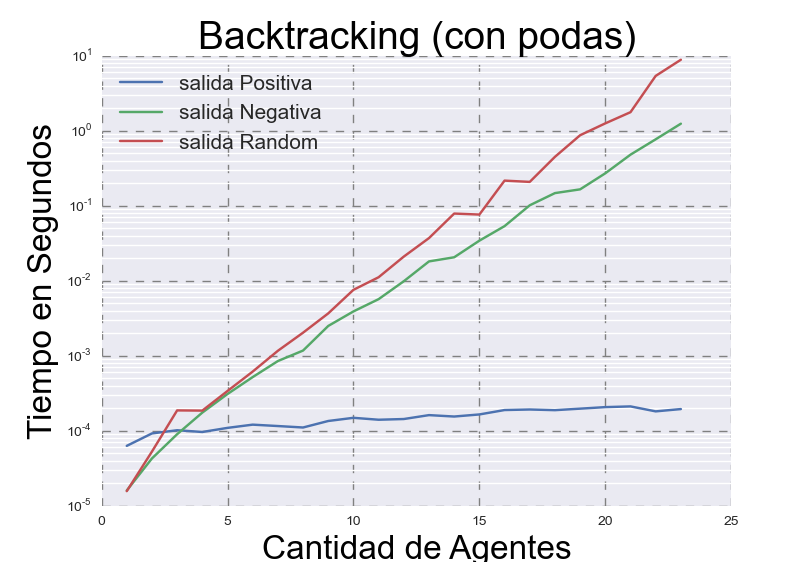
\includegraphics[scale=0.45]{BacktrackingPodasLog.png}
\end{subfigure}
\begin{subfigure}{0.5\textwidth}
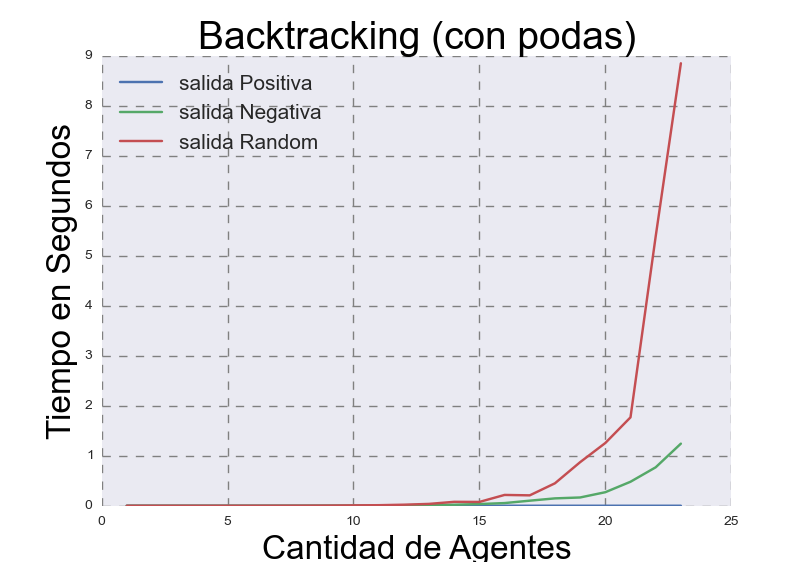
\includegraphics[scale=0.45]{BacktrackingPodas.png}
\end{subfigure}

\end{figure}

	Lo que podemos ver es que el mejor caso son las entradas positivas, esto se debe a que como la primera rama que recorre el algoritmo es determinante para la solución final, la poda que se encarga de no considerar soluciones peores o iguales poda la mayoría de las otras ramas, lo que resulta en una instancia muy buena. Mientras que las instancias random y negativas son bastantes parecidas. 
	
	Otro experimento que quisimos ver fue el mismo que vimos en la sección anterior, que consiste en fijar la cantidad de agentes e ir variando la cantidad de encuestas. La forma de generar la muestra como la forma de tomar los tiempos son iguales a las descriptas en la seccion anterior
	
	\begin{figure}[h]
	\begin{subfigure}{0.5\textwidth}
	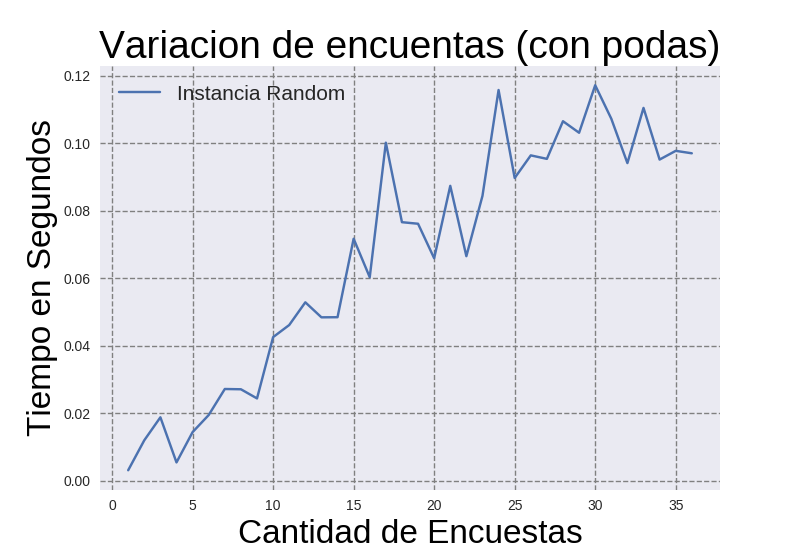
\includegraphics[scale=0.45]{VariacionesConPodas.png}
	\end{subfigure}
	\end{figure}
	
	Lo que podemos ver es que a medida que aumentamos el número de encuestas también aumenta el tiempo del algoritmo. Con lo que podemos concluir que la cantidad de encuestas afecta directamente al algoritmo. Esto se puede ver en la idea conceptual de árbol que ultilizamos antes, la idea sería que, a medida que crecen las encuestas, cuesta más pasar de un nivel a otro, ya que es ahi donde recorremos las encuestas para ver la confiabilidad de los agentes. 

\newpage

\section{Comparación}
	
	Ahora lo que nos interesa es comparar los 2 algoritmos descriptos anteriormente. La idea de esto es ver como se comportan las podas frente a no tener podas. Para esto tomamos los tiempos de ambos algoritmos sobre la entrada random descripta en las secciones anteriores. La razón por la cuál optamos por la entrada random es porque nos parece el mejor caso para comparar los algoritmos, ya que no podemos saber que se está podando y que no. Y, además, según lo que vimos antes es un mal caso para las podas, mientras que no es un caso tan malo para la versión sin podas. 

\begin{figure}[h]
\begin{subfigure}{0.5\textwidth}
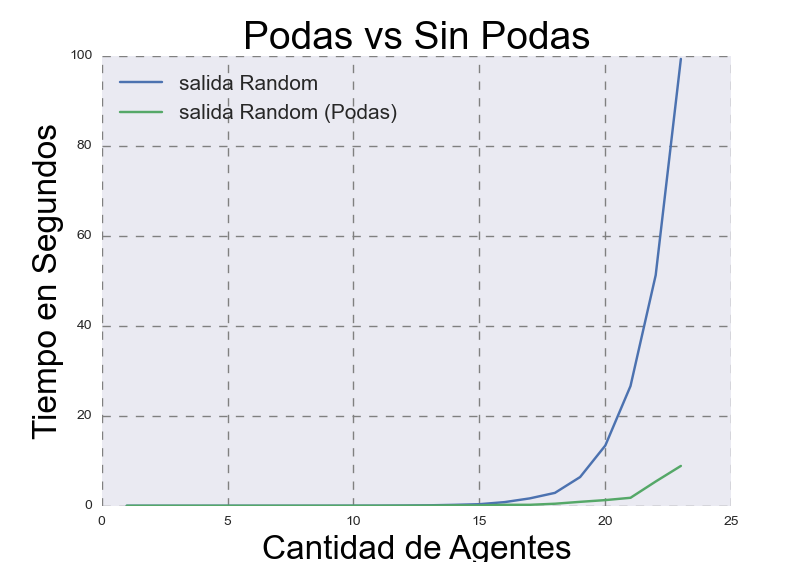
\includegraphics[scale=0.45]{Vs.png}
\end{subfigure}
\end{figure}

\begin{figure}[h]
\begin{subfigure}{0.5\textwidth}
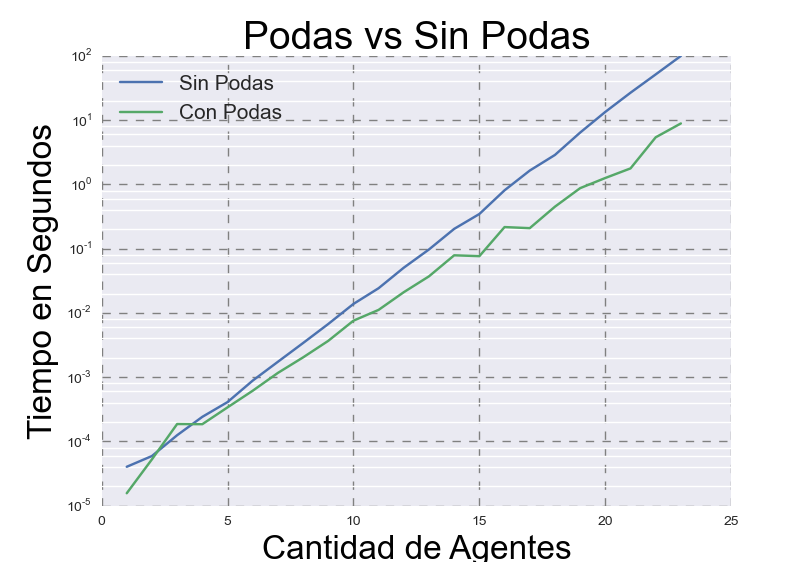
\includegraphics[scale=0.45]{VsLog.png}
\end{subfigure}
\end{figure}
	
	Lo que podemos ver en los gráficos es que el algoritmo con podas es más rápido que el que no tiene podas. Esto se debe a que las podas me ahorran recorrer ramas que no van a aportar una mejor solución al problema y, además, cuando hacemos el chequeo de si un agente es confiable, las podas hacen un chequeo más profundo que la versión sin podas.   

	

\newpage

\section{Modificaciones al informe}
	Aqui vamos a ver las diferencias con la primera entraga del trabajo.

\subsection{Backtracking}
\begin{itemize}
\setlength\itemsep{-0.2em}
\item Cambiamos la resolución del problema agregando algunos pasos que faltaban respecto de la implementación.
\item Corregimos la demostración de correctitud.
\item Se modifico la subsección de complejidad.
\item Además se agrego experimentación y se comentaron mejor los gráficos, estos últimos también fueron modificados.
\item Se modifico el pseudocódigo.
\end{itemize}

\subsection{BacktrackingPodas}
\begin{itemize}
\setlength\itemsep{-0.2em}
\item Se agrego una parte de correctitud.
\item Se agrego experimentación y una explicación sobre la misma.
\end{itemize}

\subsection{Código}
\begin{itemize}
\setlength\itemsep{-0.2em}
\item Agregamos una poda que chequea que se pueda no agregar al agente al conjunto en la parte de NoConfiable, esto lo hicimos en ambos algoritmos.
\item Se modifico el else de Confiables ya que llamaba a NoConfiable, ahora no lo hace.
\item Modificamos los pasajes a las funciones para que sean por referencia en vez de ser un puntero, se cambio el código para que respete esto.
\end{itemize}

\subsection{Comparación de algoritmos}
	Modificamos los gráficos y la explicación de los mismos.

\end{document}